% STUDENT-TEMPLATE FOR ASSIGNMENT 7 in CSE 415, UNIV. OF WASH. Winter, 2024.

\documentclass[12pt]{article}
\setlength{\oddsidemargin}{0in}
\setlength{\evensidemargin}{0in}
\setlength{\textwidth}{6.5in}
\setlength{\textheight}{8.0in}
\setlength{\parindent}{0in}
\setlength{\parskip}{\baselineskip}

\usepackage{amsmath,amsfonts,amssymb, centernot, graphicx, hyperref}
\usepackage{enumerate,color, multicol,fancyhdr,float,booktabs,calc}
\newlength\longanswerwidth
\setlength{\longanswerwidth}{\textwidth-0.8cm}


\newenvironment{qparts}{\begin{enumerate}[{(}a{)}]}{\end{enumerate}}
\newenvironment{qsubparts}{\begin{enumerate}[{(}i{)}]}{\end{enumerate}}
\newcommand\independent{\protect\mathpalette{\protect\independenT}{\perp}}
\def\independenT#1#2{\mathrel{\rlap{$#1#2$}\mkern2mu{#1#2}}}

\newcommand{\answerInBox}[2]{\fbox{\begin{minipage}{#1}\textcolor{blue}{#2}\end{minipage}}}

\usepackage{array} % For centered fixed-width cells in tabular, in Q3.
\newcolumntype{P}[1]{>{\centering\arraybackslash}p{#1}}


\title{Assignment 7 in CSE 415, Winter 2024}
\author{by the Staff of CSE 415}
\date{}
\pagestyle{fancy}
\fancyhf{}
\renewcommand{\headrulewidth}{0.4pt}% Default \headrulewidth is 0.4pt
\renewcommand{\headheight}{14.9pt}% Default \footrulewidth is 0pt
\fancyhead[L]{CSE 415, A7, Wi'2024 -- Last Name: \mbox{\textcolor{blue}{Labbe,}\hspace{0.5 in}} First Name: \mbox{\textcolor{blue}{Alexandre}} \hfill \thepage }
\renewcommand{\footrulewidth}{0.4pt}% Default \footrulewidth is 0pt
\fancyfoot[C]{Paul G. Allen School of Computer Science and Engineering, University of Washington}
\renewcommand{\headrulewidth}{0.4pt}% Default \headrulewidth is 0.4pt
\renewcommand{\headheight}{15pt}% Default \footrulewidth is 0pt
\def\independenT#1#2{\mathrel{\rlap{$#1#2$}\mkern2mu{#1#2}}}

\begin{document}
\maketitle
This is due Wednesday, March 6 via Gradescope at 11:59 PM. Prepare a PDF file with your answers and
upload it to Gradescope.
The PDF file can created however you like. For example it can be
from a scan of a printout of the assignment document onto which you
have hand-written your answers.  Or it can be from Word or Latex file
with your answers. It can even be from photos of your handwritten
answers on plain paper.  You don't have to include the questions
themselves, but it is fine to do so.
In any case, it must be very clear to read,
and it must be obvious and easy for each grader where to find your
solutions to the exercises.

As with Assignment 4, this is an
  {\it individual work} assignment.  Collaboration is not permitted.

Prepare your answers in a neat, easy-to-read
PDF.
If you choose to typeset your answers
in Latex using the template file for this document,
please put your answers in \textcolor{blue}{blue} while
leaving the original text black.

Do the following exercises.  These are intended to take
15-30 minutes each if you know how to do them. Each is worth
20 points. The total of possible points is 100.

If corrections or clarifications to the problems have to be given,
this will happen in the ED discussion forum under topic ``Assignment 7."


\vspace{1cm}
Last name: \textcolor{blue}{Labbe}, first name: \textcolor{blue}{Alexandre}

\vspace{1cm}
Student number: \textcolor{blue}{2377032}

\newpage
%------------
% Question 1
%------------
\section{Markov Models }

 (20 points) Consider the Markov Model for
the stock market shown below.

\begin{center}
  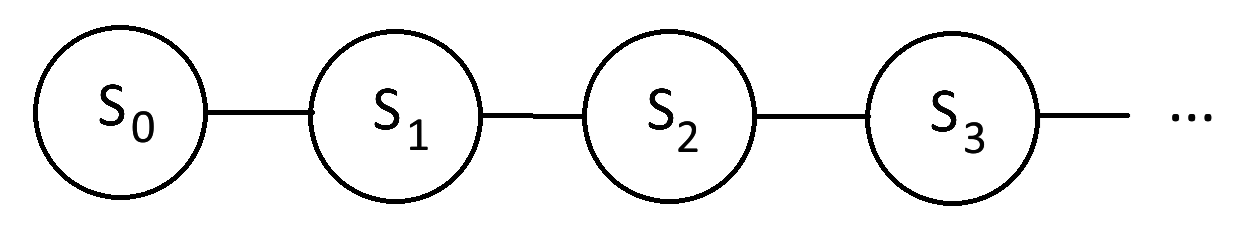
\includegraphics[width=2in]{MM-for-stocks.png}
\end{center}
The transition probabilities for this model are given as:

\begin{center}
  \begin{tabular}{||c|c|c||}
    \hline
    $S_t$   & $S_{t+1}$ & $P(S_{t+1} | S_t)$ \\
    \hline\hline
    rising  & rising    & 0.65               \\
    \hline
    rising  & falling   & 0.35               \\
    \hline
    falling & rising    & 0.5                \\
    \hline
    falling & falling   & 0.5                \\
    \hline
  \end{tabular}
\end{center}


\begin{qparts}
  \item (5 points)
  Assume $P(S_0=\mbox{rising})=1.0$ and
  $P(S_0=\mbox{falling})=0.0$.
  Using the miniforward algorithm,
  compute the $P(S_2)$ distribution.\\
  \textcolor{blue}{$P(S_2=\mbox{rising}) = 0.5975$\\
    $P(S_2=\mbox{falling}) = 0.4025$}
  \vspace{1em}

  \item (2 points)
  Continuing with the miniforward algorithm,
  compute the $P(S_3)$ distribution.\\
  \textcolor{blue}{$P(S_3=\mbox{rising}) = 0.5896$\\
    $P(S_3=\mbox{falling}) = 0.4104$}
  \vspace{1em}

  \item (3 points)
  Now assume $P(S_0=\mbox{rising})=0.0$ and
  $P(S_0=\mbox{falling})=1.0$.
  Compute the $P(S_2)$ distribution.\\
  \textcolor{blue}{$P(S_2=\mbox{rising}) = 0.5862$\\
    $P(S_2=\mbox{falling}) = 0.4138$}

  \vspace{3em}


  \item (10 points) Compute the stationary
  distribution $P(S_{\infty})$.  Show your
  work.
  \textcolor{blue}{
    \begin{align*}
      P(S_\infty=\mbox{falling}) & = P(\mbox{F}|\mbox{R}) \cdot P(S_\infty=\mbox{R}) + P(\mbox{F}|\mbox{F}) \cdot P(S_\infty=\mbox{F}) \\
                                 & = 0.35 \cdot P(S_\infty=\mbox{R}) + 0.5 \cdot P(S_\infty=\mbox{F})                                  \\
                                 & = 0.7 \cdot P(S_\infty=\mbox{R})                                                                    \\
    \end{align*}
    and
    \begin{align*}
      P(S_\infty=\mbox{falling}) + P(S_\infty=\mbox{rising}) & = 1 \\                                                             \\
    \end{align*}
    so
    \begin{align*}
      0.7 \cdot P(S_\infty=\mbox{rising}) + P(S_\infty=\mbox{rising}) & = 1               \\
      P(S_\infty=\mbox{rising})                                       & = \frac{1}{1.7}   \\
      P(S_\infty=\mbox{falling})                                      & = \frac{0.7}{1.7} \\
    \end{align*}
    Therefore,\\
    $P(S_\infty=\mbox{rising}) = 0.588\\P(S_\infty=\mbox{falling}) = 0.412$
  }

  \vspace{5em}


\end{qparts}

\newpage
%------------
% Question 2
%------------
\section{D-Separation }
 (20 points)
Consider the Bayes Net graph $\beta$ below, which represents the topology of a web-server security model. Here the random variables have the following interpretations:
\begin{description}
  \item [V]  =  Vulnerability exists in web-server code or configs.
  \item [C] =  Complexity to access the server is high. (Passwords, 2-factor auth., etc.)
  \item [S] = Server accessibility is high.  (Firewall settings, and configs on blocked IPs are permissive).
  \item [A] = Attacker is active.
  \item [L] = Logging infrastructure is state-of-the-art.
  \item [E] = Exposure to vulnerability is high.
  \item [D] = Detection of intrusion attempt.
  \item [B] = Break-in; the web server is compromised.
  \item [I] = Incident response is effective.
  \item [F] = Financial losses are high (due to data loss, customer dissatisfaction, etc).
\end{description}

\begin{center}
  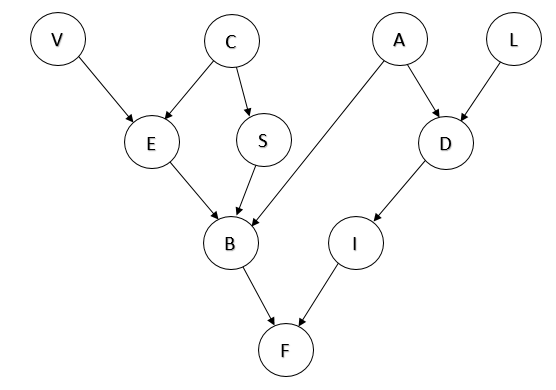
\includegraphics[width=0.6\textwidth]{D-Sep-Web-Server-Security.png}\end{center}
Let $\beta'$ be the undirected graph obtained from $\beta$ by removing the arrowheads from the edges of $\beta$.  By an ``undirected path" in $\beta$ we mean any path in $\beta'$. A ``loop-free'' path is any path in which no vertex is repeated.

\begin{qparts}
  \item (5 points) List all loop-free undirected paths from A to C in the graph $\beta$.

  \textcolor{blue}{
    $A\rightarrow B\rightarrow S\rightarrow C$\\
    $A\rightarrow B\rightarrow E\rightarrow C$\\
    $A\rightarrow D\rightarrow I\rightarrow F\rightarrow B\rightarrow E\rightarrow C$\\
    $A\rightarrow D\rightarrow I\rightarrow F\rightarrow B\rightarrow S\rightarrow C$}

  \item (5 points) Suppose random variables F and S are observed, and no others are observed.  Then which (if any) of those paths would be active paths?  Justify your answer.

  \textcolor{blue}{$A\rightarrow B\rightarrow E\rightarrow C$ Justification: ABE: collider-descendant, BEC: casual chain\\
    $A\rightarrow D\rightarrow I\rightarrow F\rightarrow B\rightarrow E\rightarrow C$ Justification: ADI: casual chain, DIF: casual chain, IBF: collider observed, FBE: casual chain, BEC: casual chain}

\end{qparts}

For each of the following statements, indicate whether (True) or not (False) the topology of the net guarantees that that the statement is true.  If False, identify a path (``undirected") through which influence propagates between the two
random variables being considered. (Be sure that the path follows the D-Separation rules covered in lecture.)
The first one is done for you.

(c) $C \independent A$: \textcolor{blue}{True (both are roots and no common descendants have been observed) }


(d) (1 point) $B \independent I \,|\, A$ \textcolor{blue}{False, BFI}

(e) (1 point) $V \independent D \,|\, E, B$ \textcolor{blue}{False, VECSBAD}

(f) (1 point) $C \independent D \,|\, A, I$ \textcolor{blue}{True}

(g) (1 point) $C \independent L \,|\, V,E,F, I$ \textcolor{blue}{True}

(h) (1 point) $V \independent F \,|\,E, B$ \textcolor{blue}{False, VECSBADIF}

(i) (5 points) Suppose that the company hired an outside expert to
examine the system and she determines that B,
E, and I are true: a Break-in has occurred (the web server is compromised), Exposure to vulnerability is high, and Incident
response is effective.  Given this
information, your job is to explain to management why getting additional
information about C (Complexity to access the server is high) could have an impact on
the probability of L (logging infrastructure
is state-of-the-art).  Give your explanation, for the manager of the company,
using about 3 to 12 lines of text, which should be based on
what you know about D-separation, applied to this situation.  However,
your explanation should not use the terminology of D-separation but be in plain English.
(You can certainly use words like ``influence", ``probability", ``given",
but not ``active path", ``triple", or even ``conditionally independent").

\textcolor{blue}{Gaining information about the complexity, allows us to make assumptions about the server accessibility. Since both the presence of an Attacker
  and the server accessibility affect our belief of whether or not a break in has occured, but we know that there has been a break in, we can begin to make assumptions about the presence of an attacker based on what we learn about the server accessibility.
  In a somewhat similar fashion, since the presence of a break in affects our belief of an attacker being active, we can begin to make assumptions about the detection of an intrusion attempt.
  Normally, we would not be able to make assume that the presence of an attacker can change influence the belief in the logging infrastructure, but since the probability of the incident response being effective changes our belief in the ability to detect intruders,
  we can now confirm this notion for the same reason that we can assume that the server accessibility can affect the belief in the presence of an attacker.}


\newpage
%------------
% Question 3
%------------
\section{Reinforcement Learning}
Use the Markov Decision Process (MDP) diagram below to help you as you answer the following questions about Value Iteration and Q Learning.

\bgroup
\def\arraystretch{3}

\begin{table}[!h]
  \centering
  %\begin{tabular}{|p{1.5cm}|p{1.5cm}|p{1.5cm}|p{1.5cm}|p{1.5cm}|p{1.5cm}|p{1.5cm}|}
  \begin{tabular}{|P{1.5cm}|P{1.65cm}|P{1.5cm}|P{1.5cm}|P{1.5cm}|P{1.5cm}|P{1.65cm}|}
    \hline
    $A$ & $B$ $(-10)$ & $C$ & $D$ & $E$ & $F$ & $G$ (+10) \\ \hline
  \end{tabular}
\end{table}
\egroup

\begin{qparts}
  \item (10 points) Use Q Learning to estimate the true q values of this MDP given the observed state transitions below. For each state transition, indicate which q value is changing by giving the state and action associated with that value and giving its new value. You may wish to keep your own diagram of the current values while you work through the given transitions.

  You may assume that at states $\{A, C, D, E, F\}$ there are two allowed actions, \{Left, Right\}, at states $\{B, G\}$, the only allowable action is the Exit action, and at the Terminal state there are no valid actions. Make sure to process the transitions in the order provided. All Q values are initialized to 0. Use a discount factor of $\gamma=0.8$ and a learning rate of $\alpha=0.5$.

  Note that although a description of the MDP parameters are given in the next part of this question, Q Learning does not rely on knowing these parameters and this problem may not use the same rules and parameters.


  \begin{table}[!h]
    \centering
    \begin{tabular}{l|l|l|l|l|l|l}
      \multicolumn{4}{l|}{State Transitions} & \multicolumn{3}{l}{New Q Values}                                                                                                         \\
      State (s)                              & Action (a)                       & New State (s') & Reward (r) & State               & Action                  & Q(S,A)                  \\ \hline
      A                                      & Right                            & B              & $-1$       & \textcolor{blue}{A} & \textcolor{blue}{Right} & \textcolor{blue}{-0.5}  \\ \hline
      B                                      & Exit                             & Terminal       & $-10$      & \textcolor{blue}{B} & \textcolor{blue}{Exit}  & \textcolor{blue}{-5}    \\ \hline
      E                                      & Right                            & D              & $-1$       & \textcolor{blue}{E} & \textcolor{blue}{Right} & \textcolor{blue}{-0.5}  \\ \hline
      D                                      & Right                            & E              & $-1$       & \textcolor{blue}{D} & \textcolor{blue}{Right} & \textcolor{blue}{-0.5}  \\ \hline
      E                                      & Right                            & F              & $-1$       & \textcolor{blue}{E} & \textcolor{blue}{Right} & \textcolor{blue}{-0.75} \\ \hline
      F                                      & Right                            & G              & $-1$       & \textcolor{blue}{F} & \textcolor{blue}{Right} & \textcolor{blue}{-0.5}  \\ \hline
      G                                      & Exit                             & Terminal       & 10         & \textcolor{blue}{G} & \textcolor{blue}{Exit}  & \textcolor{blue}{5}     \\ \hline
    \end{tabular}
  \end{table}


  \item (10 points) Value Iteration:

  Consider an MDP with the states shown in the diagram above. In this MDP, there are two allowable actions for non-goal states, \{Left, Right\}, whose intended effect is to move the agent to the state directly to the left or right of the current state respectively. However, at each action with probability $\eta$ (noise), the agent will instead move to the state in the opposite direction of its intended move. If at any point an action would move the agent to an invalid state, the agent instead will remain in place.

  At states $B$ and $G$, the only allowable action is the Exit action, which gives the reward indicated in the diagram and moves the agent to the Terminal state, which is a state with no allowable actions, indicating the end of the episode.

  A few examples with $\eta=0.3$: from state $D$, taking action Right, the agent will move to state $E$ with probability 0.7 and will move to state $C$ with probability 0.3. From state $A$, taking action Left, the agent will remain in state $A$ with probability 0.7 and will move to state $B$ with probability 0.3. From state $B$, the only allowed action is Exit, which gives reward $-10$.

  Perform three iterations of value iteration on the MDP described above, using noise $\eta=0.2$, discount $\gamma=0.9$, and a living reward of 0.0. The initial values, $V_0$, for all the states are provided for you. Write the values $V_i$ corresponding to each state in the boxes for that state for iterations $i=1, 2, 3$.

  $V_0$:

  \bgroup
  \def\arraystretch{3}
  \begin{tabular}{|p{1.5cm}|p{1.5cm}|p{1.5cm}|p{1.5cm}|p{1.5cm}|p{1.5cm}|p{1.5cm}|}
    \hline
    $A$: 0 & $B$: 0 & $C$: 0 & $D$: 0 & $E$: 0 & $F$: 0 & $G$: 0 \\ \hline
  \end{tabular}
  \egroup

  $V_1$:

  \bgroup
  \def\arraystretch{3}
  \centering
  \begin{tabular}{|p{1.5cm}|p{1.5cm}|p{1.5cm}|p{1.5cm}|p{1.5cm}|p{1.5cm}|p{1.5cm}|}
    \hline
    $A$ \underline{\textcolor{blue}{0}} & $B$ \underline{\textcolor{blue}{-10}} & $C$ \underline{\textcolor{blue}{0}} & $D$ \underline{\textcolor{blue}{0}} & $E$ \underline{\textcolor{blue}{0}} & $F$ \underline{\textcolor{blue}{10}} & $G$ \underline{\textcolor{blue}{0}} \\ \hline
  \end{tabular}
  \egroup

  $V_2$:

  \bgroup
  \def\arraystretch{3}
  \centering
  \begin{tabular}{|p{1.5cm}|p{1.5cm}|p{1.5cm}|p{1.5cm}|p{1.5cm}|p{1.5cm}|p{1.5cm}|}
    \hline
    $A$ \underline{\textcolor{blue}{-1.8}} & $B$ \underline{\textcolor{blue}{-10}} & $C$ \underline{\textcolor{blue}{-1.8}} & $D$ \underline{\textcolor{blue}{0}} & $E$ \underline{\textcolor{blue}{7.2}} & $F$ \underline{\textcolor{blue}{10}} & $G$ \underline{\textcolor{blue}{7.2}} \\ \hline
  \end{tabular}
  \egroup

  $V_3$:

  \bgroup
  \def\arraystretch{3}
  \centering
  \begin{tabular}{|p{1.5cm}|p{1.5cm}|p{1.5cm}|p{1.5cm}|p{1.5cm}|p{1.5cm}|p{1.5cm}|}
    \hline
    $A$ \underline{\textcolor{blue}{-3.096}} & $B$ \underline{\textcolor{blue}{-10}} & $C$ \underline{\textcolor{blue}{-1.8}} & $D$ \underline{\textcolor{blue}{4.86}} & $E$ \underline{\textcolor{blue}{7.2}} & $F$ \underline{\textcolor{blue}{10}} & $G$ \underline{\textcolor{blue}{8.496}} \\ \hline
  \end{tabular}
  \egroup


\end{qparts}

\newpage
%------------
% Question 4
%------------
\section{ The Laws of Robotics }
 (20 points) In the 1940's, Isaac Asimov introduced a set of three laws to govern robot behavior:
\begin{enumerate}
  \item A robot may not injure a human being or, through inaction, allow a human being to come to harm.
  \item A robot must obey the orders given it by human beings except where such orders would conflict with the First Law.
  \item A robot must protect its own existence as long as such protection does not conflict with the First or Second Laws.
\end{enumerate}

(NOTE: You might also want to take a look at this cartoon \url{https://xkcd.com/1613/})

For this question, you will read Asimov's short story \textit{Liar!} linked here:\\
\url{https://courses.cs.washington.edu/courses/cse415/24wi/uwnetid/misc/Asimov-Liar.pdf}.

It is one of Asimov's robot short stories that were collected together in the book \textit{I, Robot}. After you have read the story, please answer the questions below.

\begin{qparts}
  \item (1 points) Who was Isaac Asimov and what is his relevance to the field of Artificial Intelligence (answer in 3-4 sentences)?

  \textcolor{blue}{Issac Asimov was a science fiction writer. He coined the term "robotics" and introduced the three laws of robotics. These laws are ethical principals for designing intelligent robots, which can be looked at as guidelines for designing artificial intelligence systems.}
  \vspace{3cm}

  \item (2 points) Explain why the robot was lying to the humans in the story.\\

  \textcolor{blue}{The robot can read minds, therefore it is able to know what the humans want to hear and do not want to hear. The robot makes the assumption that telling a human something it does not want to hear, then it would be hurting the human. So, when the robot has garnered knowledge by reading the thoughts of other humans, and learns information about that a human does not want to hear, it does not tell the human the human the truth because it has assumed that telling the human the truth would be hurting it. The robot is acting in accordance to the first law of robotics, which takes priority over all other rules.}

  \vspace{1cm}

  \item (2) Do you think the robot behaved in accordance to the Laws of Robotics by lying or should it have realized that lying could also lead to harm being done (remember to explain your reasoning)?\\

  \textcolor{blue}{I do think the robot was behaving in accordance to the Laws of Robotics. The robot made the assumption that telling the human something it does not want to hear, then it would be hurting the human. The robot had to make a decision, is lying or telling the truth more harmful to the human. It decided the truth was more harmful. Although I do not agree with this line of thought, I understand why the robot has adopted it. It decided early on that lying was better, and it had to stick by its line of reasoning and continue to lie to humans.}

  \vspace{1cm}

  \item (4 points) Brain-computer interfaces are an area of active research today. What are some beneficial applications of these technologies (if you look online to help you answer this question, please include citations)? \\

  \textcolor{blue}{A beneficial application of these technologies is supplementing a compromised portion of a humans brain. If a human's brain is no longer, or never was, able to perform certain tasks, some would want to be able to supplement that function of the brain through brain-computer interfaces.}

  \vspace{1cm}

  \item (4 points) What are some concerns you would have with technology that could in some way "read" the user's mind (cite any references you consult)?

  \textcolor{blue}{In a world where everything is becoming digital, where everything can be posted, where even the private information we store online is at risk of being made public, our thoughts are the only things we have left that we can keep private. For as long as we live, or until the introduction of mind reading technology, we have the right to keep our thoughts private. Our actions are rarely reflective of our thoughts. But does that even matter? After all it is only based upon our actions that our character can be judged upon. It should stay that way, allowing us to keep our thoughts private as they are ours and ours only.}

  \vspace{1cm}


  \item (1 points) Keeping in mind the requirement that the robot has to obey the Laws of Robotics, did you find the end of the story effective and/or convincing? Explain why or why not.

  \textcolor{blue}{I did find the end of the story effective. The robot was put into a situation where it had two options, and both options would result in hurting a human. By following the orders of the humans (Law 2), it would hurt the humans. But by not following the orders, it was also hurting the human. The robot had no other option than to break.}

  \vspace{1cm}

  \item (3 points) If you were creating a mind-reading robot today, how might you try to program the robot to prevent such a catastrophic result? In your response, assume you are free to modify or eliminate the laws of robotics. \\

  \textcolor{blue}{Following the sentiment I described earlier, I would not create a robot that could read minds. But in spirit of the question, I would allow the robot to read minds, but not to share the things it has learned to other people. I would allow the robot to communicate about thoughts only with the owner of the thoughts.}

  \vspace{1cm}

  \item (3 points) Did the approach you described above require modifications to or the elimination of the laws of robotics? Do you think constraints at the hardware (e.g. robot) level are the correct approach to take to ensuring ethical uses of technology? Explain why or why not.

  \textcolor{blue}{I could implement my ideas by changing some of the laws of robotics. I would add an addendum to Law number 1, stating that sharing information that a human deems private is grounds for hurting the human. This would force the robot to not share private information because it would be harming the human. I do not think hardware constraints are the correct approach, I think this has to be done at the software level because if the software has no constraints, it could bypass the physical constraints in some ways.}


\end{qparts}


\newpage
%------------
% Question 5
%------------
\section{Perceptrons}
 (20 points) In this question we'll assume that
perceptrons should output $1$ if  $ \sum_{i=0}^{n} w_i x_i \geq 0$ and 0 otherwise. The weight $w_0$ is called the bias weight, and $x_0$ is called the bias input and it is always equal to 1.
\begin{qparts}
  \item (4 points) Assuming there will be two inputs $x_1$ and $x_2$, each with possible values in $\{0,1\}$, give values for a triple of weights $\langle w_0,w_1,w_2 \rangle$  such that the corresponding perceptron would act as
  a NOR
  gate for the two inputs. (Again, weight $w_0$ is the bias weight.) Note that a
  NOR
  gate outputs 1 when both its inputs are 0;
  it outputs 0 otherwise.
  \vspace{0.5cm}

  \textcolor{blue}{$\langle 1,-2,-2 \rangle$}

  \item (4 points)  Draw a perceptron, with weights, that accepts a single integer $x_1$ and outputs 1 if and only if the input is greater than or equal to $-5$. Be sure to include $x_0$ ( the bias input of value 1) and its weight $w_0$ in your diagram.  Draw another perceptron that outputs 1 if and only if the input is less than or equal to $5$.
  \vspace{1cm}

  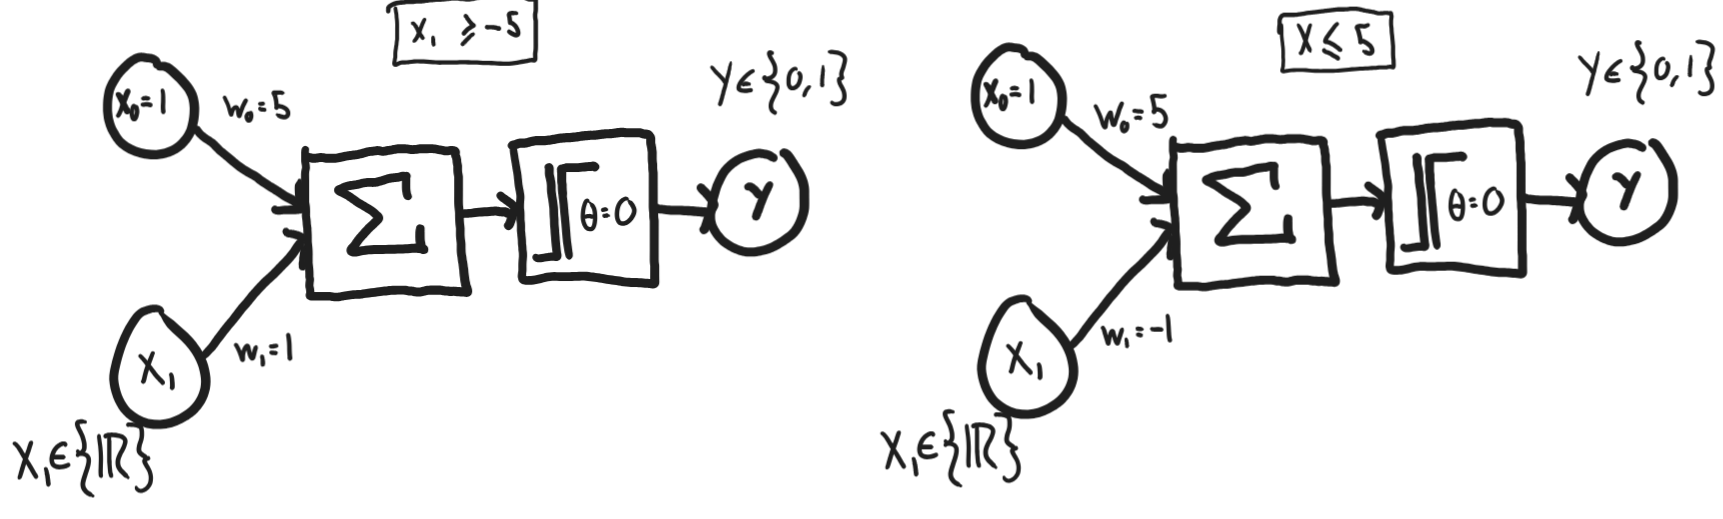
\includegraphics[width=0.8\textwidth]{Perceptrons.png}


  \item (4 points)  Using the previous perceptrons, create a two-layer perceptron that outputs 1
  if $|x| \le 5$, and 0 otherwise.
  \vspace{1.5cm}

  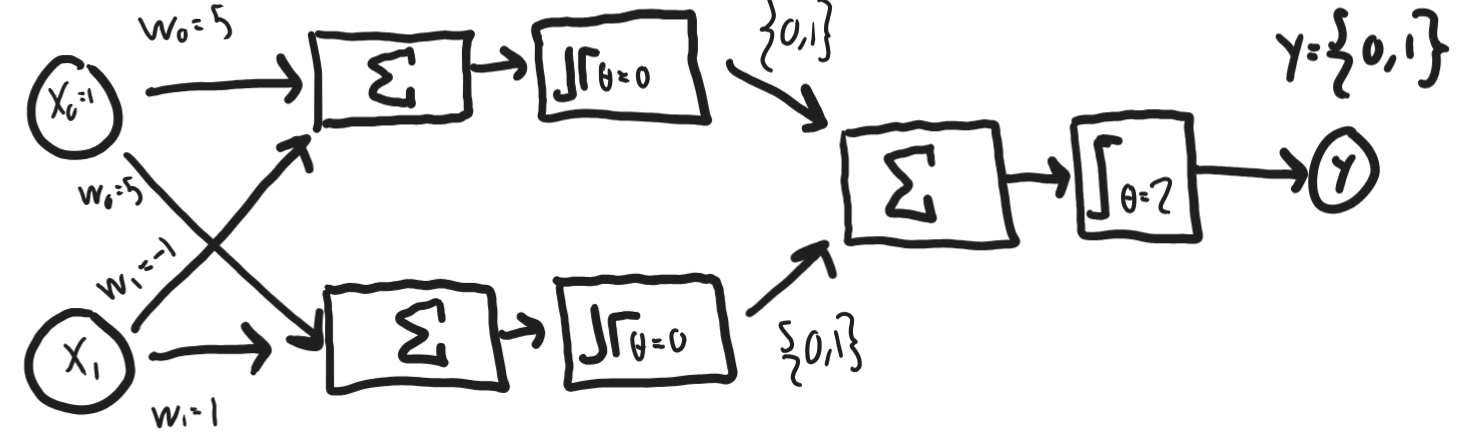
\includegraphics[width=0.8\textwidth]{2-layer.png}

  \item (4 points) Suppose we want to train a perceptron to compare two numbers $x_1$ and $x_2$ and produce output $y=1$ provided that $x_2$ exceeds $x_1$ by at least 7.
  Assume that the initial weight vector is: $\langle w_0, w_1, w_2\rangle = \langle 1, -1, -1 \rangle$.
  Consider a first training example: $(\langle x_1, x_2 \rangle, y) = (\langle 3, 11 \rangle, 1)$.  This says that with inputs 3, and 11, the output $y$ should be 1, since 11 exceeds 3 by 8.
  What will be the new values of the weights after this training example has been processed one time?  Assume the learning rate is 2.
  \vspace{1.0cm}

  \textcolor{blue}{$\langle w_0, w_1, w_2\rangle = \langle 3, 5, 21 \rangle$.}

  \item (4 points) Continuing with the last example, now suppose that the next step of training involves a different training example:
  $(\langle 2, 8 \rangle, 0)$.  The output for this example should be 0,  since 8 does not exceed 2 by at least 7.
  Starting with the weights already learned in the first step,
  determine what the adjusted weights should be after this new example has also been processed
  once.

  \textcolor{blue}{$\langle w_0, w_1, w_2\rangle = \langle 2, 3, 13 \rangle$.}


\end{qparts}

\end{document}